\documentclass[]{article}
\usepackage{lmodern}
\usepackage{amssymb,amsmath}
\usepackage{ifxetex,ifluatex}
\usepackage{fixltx2e} % provides \textsubscript
\ifnum 0\ifxetex 1\fi\ifluatex 1\fi=0 % if pdftex
  \usepackage[T1]{fontenc}
  \usepackage[utf8]{inputenc}
\else % if luatex or xelatex
  \ifxetex
    \usepackage{mathspec}
  \else
    \usepackage{fontspec}
  \fi
  \defaultfontfeatures{Ligatures=TeX,Scale=MatchLowercase}
\fi
% use upquote if available, for straight quotes in verbatim environments
\IfFileExists{upquote.sty}{\usepackage{upquote}}{}
% use microtype if available
\IfFileExists{microtype.sty}{%
\usepackage{microtype}
\UseMicrotypeSet[protrusion]{basicmath} % disable protrusion for tt fonts
}{}
\usepackage[margin=1in]{geometry}
\usepackage{hyperref}
\hypersetup{unicode=true,
            pdfborder={0 0 0},
            breaklinks=true}
\urlstyle{same}  % don't use monospace font for urls
\usepackage{longtable,booktabs}
\usepackage{graphicx,grffile}
\makeatletter
\def\maxwidth{\ifdim\Gin@nat@width>\linewidth\linewidth\else\Gin@nat@width\fi}
\def\maxheight{\ifdim\Gin@nat@height>\textheight\textheight\else\Gin@nat@height\fi}
\makeatother
% Scale images if necessary, so that they will not overflow the page
% margins by default, and it is still possible to overwrite the defaults
% using explicit options in \includegraphics[width, height, ...]{}
\setkeys{Gin}{width=\maxwidth,height=\maxheight,keepaspectratio}
\IfFileExists{parskip.sty}{%
\usepackage{parskip}
}{% else
\setlength{\parindent}{0pt}
\setlength{\parskip}{6pt plus 2pt minus 1pt}
}
\setlength{\emergencystretch}{3em}  % prevent overfull lines
\providecommand{\tightlist}{%
  \setlength{\itemsep}{0pt}\setlength{\parskip}{0pt}}
\setcounter{secnumdepth}{0}
% Redefines (sub)paragraphs to behave more like sections
\ifx\paragraph\undefined\else
\let\oldparagraph\paragraph
\renewcommand{\paragraph}[1]{\oldparagraph{#1}\mbox{}}
\fi
\ifx\subparagraph\undefined\else
\let\oldsubparagraph\subparagraph
\renewcommand{\subparagraph}[1]{\oldsubparagraph{#1}\mbox{}}
\fi

%%% Use protect on footnotes to avoid problems with footnotes in titles
\let\rmarkdownfootnote\footnote%
\def\footnote{\protect\rmarkdownfootnote}

%%% Change title format to be more compact
\usepackage{titling}

% Create subtitle command for use in maketitle
\newcommand{\subtitle}[1]{
  \posttitle{
    \begin{center}\large#1\end{center}
    }
}

\setlength{\droptitle}{-2em}

  \title{}
    \pretitle{\vspace{\droptitle}}
  \posttitle{}
    \author{}
    \preauthor{}\postauthor{}
    \date{}
    \predate{}\postdate{}
  
\usepackage{graphicx,latexsym}
\usepackage{amssymb,amsthm,amsmath}
\usepackage{longtable,booktabs,setspace}
\usepackage{mathtools}

\begin{document}

\section{Model Specification and
Results}\label{model-specification-and-results}

The goal of this chapter is apply inferential statistical modeling to
the data. This task can be divided into three steps: specifying the
models mathematically, fitting the models, and interpreting the
results\footnote{In theory there is also the step of translating the
  models from their mathematical specification into some sort of
  algorithmic process that produces estimates of coefficients and error
  terms. This process is arduous and long, so it is not included in this
  chapter. Appendix A deals with some of the techniques involved with
  model estimation}. However, before jumping into this process, it is
worth going into some key problems with the models produced. As a
consequence of these issues, some of the models are not estimated to the
standards of convergence that are commonly set.

\subsection{Modelling Issues}\label{modelling-issues}

\subsubsection{Lack of variability}\label{lack-of-variability}

To put it very simply, it's not enough to have hundreds of thousands of
observations if they are all almost identical to each other. If, for
example, my data included a thousand people in Jefferson county, and 63
in all other counties of Colorado combined (one in each remaining
county), then I would not be able to leverage my data to draw
conclusions on county-level effects.

As previously stated, the data available includes registration files
going back to 2012. From these files, I have extracted data for
elections going back to 2010 \footnote{See section 3.3.1; the extracted
  data is limited to this time period to avoid accuracy issues with
  migration and removal of inactive/unavailable voters.}. In order to
make inferences on VBM and turnout effects it is necessary to have
extensive and varied data. Specifically, it is necessary to have data
that include a large enough sample of the voters in Colorado, with a
substantial portion of them using different voting methods, from
different counties, or in different election years etc.

The data are extensive (over 35 million observations at the individual
level) but substantially lack variance in voting method. Put simply, the
vast majority of registrants in Colorado from 2010 onward either did not
vote at all, or voted by mail. If you recall the changes in Colorado
election law, in 2008 counties were allowed to conduct all mail
elections, and no-excuse permanent absentee voting was implemented
state-wide; then in 2013 Colorado transitioned to full VBM for all
elections. This means that few people were still using traditional
polling places or vote centers to cast their ballots. Figure 4.1 shows
how, after 2013, and even before that in 2011--the coordinated, local
election for which mail ballots were more convenient for counties--over
95\% of ballots cast were mail ballots. Only in the general elections of
2010 and 2012 is there some variance, but mail ballots account for well
over two thirds of total votes.

\begin{figure}

{\centering 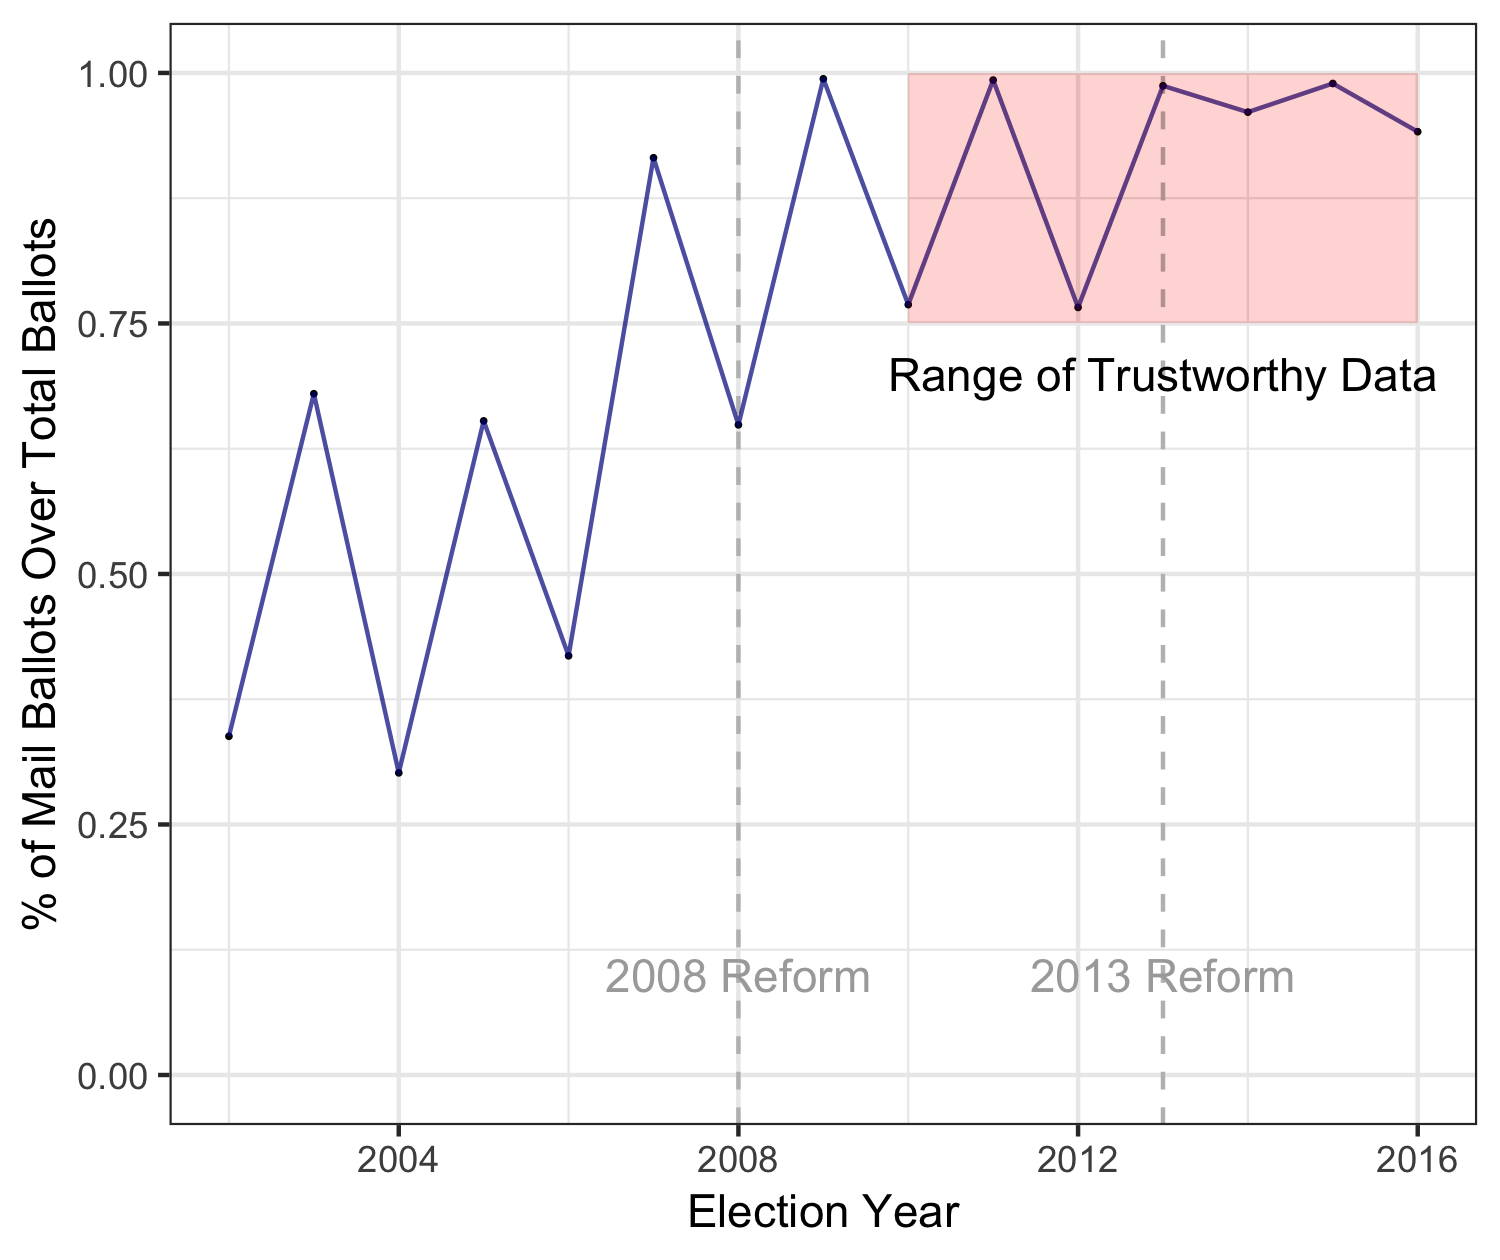
\includegraphics[width=0.8\linewidth]{/Users/tdounias/Desktop/Reed_Senior_Thesis/plots/vbm_county_graph} 

}

\caption{Percentage of mail ballots over total ballots by year}\label{fig:vbm png}
\end{figure}

This issue is not completely fatal for county level models. There is
still variance between counties that have 100\% mail ballots and those
that are around the 75-85\% margin. For individual level models, where I
am estimating voting probability, VBM will be an almost perfect
predictor for voting, and therefore will not present me with any
substantial analytical result on how it affects voting probability.
There are some ways to compensate for this issue, which I outline; due
to time or data constraints, not all of these will be implemented in
this thesis:

\begin{itemize}
\item
  \emph{More (Diverse) Data}: It would be very useful to get snapshot
  data of Colorado voter files from, say, 2004 to today, because it
  would allow for an extensive study on how the 2008 and 2013 election
  laws re-shaped voting decisions in the state. It would be useful, but
  also expensive and very time consuming, involving several purchases of
  data from the Secretary of State of Colorado. Voter registration files
  also tend to get messier the further back one goes, which means that
  the process of cleaning up the data would get substantially harder. It
  would also require more processing power to handle more observations.
  My research here does not do this, as the scope of a senior thesis is
  a lot more limited than such an overarching study that would probably
  be conducted by multiple researchers with several assistants. I do
  however present several replicable materials for such a study, through
  the creation of an \textit{R} package I include on my GitHub page
  along with the final results of this thesis. This thesis does not go
  that far, but it may help similar studies in the future.
\item
  \emph{Localized, Natural Experiment Studies}: A natural experiment is
  when, due to policy changes and circumstances, a ``control'' and
  ``treatment'' group of such a policy are created in the same
  approximate geographical area. This happens when, for example, only
  some of the counties in a state enact a specific change. Several such
  studies exist already, with some even tackling VBM in Colorado
  {[}@keele\_geographic\_2017{]}, or how turnout rates are affected by
  new, restrictive registration laws {[}@burden\_election\_2013{]}. This
  method would allow for more accuracy in both the individual and county
  level models, and through the existence of a treatment and control
  group would guarantee the variability that I am currently lacking.
\item
  \emph{Synthetic Control Group}: The synthetic control group method is
  a way of creating a control group when no such group seems to exist.
  It involves gathering a set of characteristics from the treatment
  group members and then using statistical methods to combine them into
  making the appropriate control {[}@mcclelland\_synthetic\_2017{]}. I
  will not go into the particulars of this method (the sources cited
  should provide a decent introduction), but this method has been
  successful in assessing policy effects such as anti-smoking laws
  {[}@barr\_comprehensive\_2012{]}, or even motor voter laws in
  Oregon{[}@gronke\_voter\_2017{]}.
\end{itemize}

\subsubsection{Computational
Considerations}\label{computational-considerations}

The process of computing estimates for model coefficients can often be
very computationally intensive. This issue was particularly present
during estimation of individual level models, which alongside complex
hierarchical structure also draw on a huge dataset of 35 million
observations. This computationally intensive procedure requires more
processing power than I currently have available. For now, I compensated
for this problem by using stratified sampling to sample a subset of my
observations\footnote{A long term solution to this issue could be the
  use of a more powerful local RStudio server, or Amazon Web Services
  (AWS).}.

The form of stratified sampling I am using is very simple; based on
county, mail vote, and electoral participation, I use \texttt{dplyr} in
\textit{R} to draw a sample that contains equal proportions of every
combination of values of these variables to those in the original
dataset. If, for example, the original dataset had 2\% of entries being
voters from Jefferson county that participated using a mail ballot, the
sampled dataset would have a proportion that is approximately equal to
2\% {[}@chihara\_mathematical\_2011{]}. In this way I draw a sample of
around 400,000 observations from my initial ballot dataset, on which I
run all my individual models. After checking the variable ratios in
sampled and population datasets, I found that the differences between
ratios had a mean and standard deviation of less than a hundredth of a
percentile. Therefore this sampled dataset could serve as a decent
approximation of my population.

\subsection{Variable Specification}\label{variable-specification}

I will not go through each individual variable in this section, but will
briefly describe my notation for the following models. I will include
more comments whenever they seem necessary under each model. In this
thesis I include predictors on a series of variables that can be divided
into five categories based on unit of observation: county, election,
individual, local result, and ballot. The last two are functions of
other units: local result units are equal to the product of elections
and counties, while ballot units are equal to the number of unique
individuals multiplied by the number of elections each of them was
registered in. For notation, I follow this set of rules:

\begin{enumerate}
\def\labelenumi{\arabic{enumi}.}
\tightlist
\item
  If the variable is a response, it is coded \(y\).
\item
  If the variable is a predictor, it is coded \(x\)
\item
  The variable's superscript will provide information on what it
  represents, else it will be explained.
\item
  All variables represent a single value (scalar) of that variable
  unless stated otherwise.
\item
  Unit of observation will also be specified in subscript, according to
  the indices described in Table 4.1. These indices are also used in sum
  notation.
\item
  All Greek characters represent coefficients to be calculated.
\item
  By \(k[j]\) I represent the k-value corresponding to the
  j-observation. In this case, this would be the county that an
  individual is registered in.
\item
  Note that for Local Result level variables, I use \(k,l\) as an index.
  This is because there are very few variables at this level, it is a
  direct Cartesian product of two other units, and this notation avoids
  confusion with even more index types.
\end{enumerate}

\begin{longtable}[]{@{}lc@{}}
\caption{Variable indices per unit of observation
\label{tab:units_vars}}\tabularnewline
\toprule
\begin{minipage}[b]{0.27\columnwidth}\raggedright\strut
Units\strut
\end{minipage} & \begin{minipage}[b]{0.16\columnwidth}\centering\strut
Index\strut
\end{minipage}\tabularnewline
\midrule
\endfirsthead
\toprule
\begin{minipage}[b]{0.27\columnwidth}\raggedright\strut
Units\strut
\end{minipage} & \begin{minipage}[b]{0.16\columnwidth}\centering\strut
Index\strut
\end{minipage}\tabularnewline
\midrule
\endhead
\begin{minipage}[t]{0.27\columnwidth}\raggedright\strut
Ballot\strut
\end{minipage} & \begin{minipage}[t]{0.16\columnwidth}\centering\strut
i\strut
\end{minipage}\tabularnewline
\begin{minipage}[t]{0.27\columnwidth}\raggedright\strut
Individual\strut
\end{minipage} & \begin{minipage}[t]{0.16\columnwidth}\centering\strut
j\strut
\end{minipage}\tabularnewline
\begin{minipage}[t]{0.27\columnwidth}\raggedright\strut
County\strut
\end{minipage} & \begin{minipage}[t]{0.16\columnwidth}\centering\strut
k\strut
\end{minipage}\tabularnewline
\begin{minipage}[t]{0.27\columnwidth}\raggedright\strut
Election\strut
\end{minipage} & \begin{minipage}[t]{0.16\columnwidth}\centering\strut
l\strut
\end{minipage}\tabularnewline
\begin{minipage}[t]{0.27\columnwidth}\raggedright\strut
General Index\strut
\end{minipage} & \begin{minipage}[t]{0.16\columnwidth}\centering\strut
v\strut
\end{minipage}\tabularnewline
\bottomrule
\end{longtable}

\subsection{County Level Models}\label{county-level-models}

\subsubsection{Specifications}\label{specifications}

In this section I will go through a step-by step creation of models at
the county level. County level models use a series of variables at the
election, county, and local result levels. The response variable is
always turnout in one county after a particular election. With no other
information, this model could be thought of as an assignment of voting
tendencies across counties; each county independent of election has a
unique range of turnout results. In this way it is possible to build a
naive, baseline model of turnout as follows:

\begin{equation} \tag{Model 1}
Y^{turnout}_{k,l} = \beta_0 + (\sum_{k=1}^{64}\beta_kx_k^{county}) + \epsilon,\ \epsilon \sim N(0,\sigma^2)
\end{equation}

where \(x_k^{county}\) is a series of 64 dummy variables for each county
of Colorado. Here differences between elections come from normally
distributed error terms, rather than predictors. I name this
\textbf{Model 1}, and it does not reflect the data particularly well.
First off, this model includes the assumption that counties are
independent of one another, which is probably false; just consider that
these counties are areas of the same state, in the same country, with
populations moving between them at regular intervals, and many of them
covering the same metropolitan area or congressional district.
Additionally, the model matrix here is rank deficient; there are two
county coefficients that are perfect linear combinations of other
coefficients. This means they will be dropped by \textit{R} when the
model is called in the \texttt{lm()} function.

A way to fix both these issues is to use a multilevel model with mixed
effects for county. By constraining coefficients at the county level to
a set distribution, this model does away with the assumption of
independence. The other county level predictors help to explain some of
the unexplained group level variation, which reduces the standard
deviation of county coefficients and helps provide more exact estimates
{[}@gelman\_data\_2006{]}. I call this \textbf{Model 2}, which can be
written as:

\begin{equation} \tag{Model 2}
Y^{turnout}_{k,l} = a_{k} + \beta_{1}x_k^{\%white} + \beta_{2}x_k^{\%urban} + \epsilon,
\end{equation}

\[a_{k} \sim N (\gamma_0, \sigma_{\alpha}^2)\]
\[\epsilon \sim N(0, \sigma^2)\] This model provides a more reasonable
set of estimates for each county, but still fails to provide any
information as to secular trends, time-specific effects, election type
effects, or mail voting--the variable of interest. I will amend this by
adding a set of variables at the election and local result levels:
election type and an interaction term between election type and mail
voting. This variable should reflect whether turnout effects of mail
voting are more pronounced in a specific type of election. I call this
\textbf{Model 3} and it can be specified as follows:

\begin{multline} \tag{Model 3}
Y^{turnout}_{k,l} = a_{k} + \beta_{1}x_k^{\% white} + \beta_{2}x_k^{\% urban} + \overbrace{(\sum_{v=3}^{6}\beta_{v}x_{v}^{election type} x_{k,l}^{\% mail~vote})}^\text{Interaction Effect with Type} + \\ \overbrace{(\sum_{v=7}^{10}\beta_{v}x_{v}^{election type})}^\text{Main Effect of Election Type} + \epsilon,
\end{multline}

\[a_{k} \sim N(\gamma_0, \sigma_{\alpha}^2)\]
\[\epsilon \sim N(0, \sigma^2)\]

where \(x_{v}^{election type}\) is a series of four dummy variables for
each type of election (General, Primary, Coordinated, Midterm). This
model reflects nearly all the information I have available, apart from
election date. For the incorporation of election dates there are two
possible alternatives. First, I can simply add a dummy variable for each
year. This would assume independence between each year, as it would
specify different, independent ``slopes'' for the seven years I have
data for--this is like calculating seven different models, one for each
year. This is not particularly elegant as a solution nor does it reflect
the fact that years actually are interconnected; of course there can be
massive shifts in national or regional political climates, but those
shifts happened \emph{from some baseline}, which is reflected in
previous years.

These elections can be thought of as systems for which prior condition
affects future outcomes, and therefore time cannot be modeled as a
series of independent effects. The solution here is adding a spline
function for time, using a general additive multilevel model. The most
commonly used spline function, and the default in the \texttt{gamm4}
\textit{R} package is a thin plate regression spline, which I also use
here {[}@wood\_generalized\_2006{]}. More on the subject of splines can
be found in the Wood (2006) textbook. The model, which I call
\textbf{Model 4} can be written as follows:

\begin{multline}\tag{Model 4}
Y^{turnout}_{k,l} = a_{k} + \beta_{1}x_k^{\% white} + \beta_{2}x_k^{\% urban} + \overbrace{(\sum_{v=3}^{6}\beta_{v}x_{v}^{election type} x_{k,l}^{\% mail~vote})}^\text{Interaction Effect with Type} + \\ \overbrace{(\sum_{v=7}^{10}\beta_{v}x_{v}^{election type})}^\text{Main Effect of Election Type} + s(x^{year}_{l}) + \epsilon,
\end{multline}

\[a_{k} \sim N(\gamma_0, \sigma_{\alpha}^2)\]
\[\epsilon \sim N(0, \sigma^2)\]

where \(s()\) is a natural cubic regression spline function with seven
knots--equal to the number of years.\footnote{I used the
  \texttt{gam.check()} function that is present in the \texttt{mgcv}
  \textit{R} package, whose call determined that the number of knots
  here may be too low. However, given the data available to me, I was
  limited to the inclusion of seven years and as such cannot increase
  the number of knots any further. Setting the number of knots to seven
  also gave the lowest CV MSE.} A summary of these four models is
provided in the following table:

\begin{longtable}[]{@{}ll@{}}
\caption{County level model descriptions
\label{tab:model_desc_county}}\tabularnewline
\toprule
\begin{minipage}[b]{0.15\columnwidth}\raggedright\strut
Model No\strut
\end{minipage} & \begin{minipage}[b]{0.80\columnwidth}\raggedright\strut
Model Description\strut
\end{minipage}\tabularnewline
\midrule
\endfirsthead
\toprule
\begin{minipage}[b]{0.15\columnwidth}\raggedright\strut
Model No\strut
\end{minipage} & \begin{minipage}[b]{0.80\columnwidth}\raggedright\strut
Model Description\strut
\end{minipage}\tabularnewline
\midrule
\endhead
\begin{minipage}[t]{0.15\columnwidth}\raggedright\strut
Model 1\strut
\end{minipage} & \begin{minipage}[t]{0.80\columnwidth}\raggedright\strut
Naive model with only county specific effects\strut
\end{minipage}\tabularnewline
\begin{minipage}[t]{0.15\columnwidth}\raggedright\strut
Model 2\strut
\end{minipage} & \begin{minipage}[t]{0.80\columnwidth}\raggedright\strut
Multilevel model; added county level predictors\strut
\end{minipage}\tabularnewline
\begin{minipage}[t]{0.15\columnwidth}\raggedright\strut
Model 3\strut
\end{minipage} & \begin{minipage}[t]{0.80\columnwidth}\raggedright\strut
Multilevel model; added VBM, interaction terms, and election fixed
effects\strut
\end{minipage}\tabularnewline
\begin{minipage}[t]{0.15\columnwidth}\raggedright\strut
Model 4\strut
\end{minipage} & \begin{minipage}[t]{0.80\columnwidth}\raggedright\strut
Multilevel General Additive model; added spline function for election
year\strut
\end{minipage}\tabularnewline
\bottomrule
\end{longtable}

\subsubsection{Results}\label{results}

The table in this section presents coefficients and standard errors for
all four county level models. This table does not include any metrics
for county--either mixed or fixed effects. I have chosen to omit these
because they firstly are not very relevant to my hypotheses, and
secondly because they are very extensive--64 coefficients for each of
the four models. I have also not included any metric for time--here
measured in years and used only in the fourth model. Both the mixed
effects for county and the measure for time should be considered as
controls: the first controls for county-specific trends while still
restricting these to allow for non-independence, and the second makes
sure that my results are indicative of a secular trend, accounting for
any shifts along time.

In terms of goodness-of-fit, I use 5-fold cross-validated Mean Squared
Error (MSE) for all of the models. There is a significant drop-off in
MSE between Models 1, 2 and Models 3, 4 of around \(.35\), which shows
that the variables introduced in the later models substantially increase
how well the models explain variability in the data. There is also a
small increase of CV MSE between models 3 and 4, but the numbers are
very comparable\footnote{If I was trying to make a model for predictive
  purposes I would probably choose Model 3; however, there is still
  value in comparing Models 3 and 4, even if the later doesn't fit the
  data better than 3. The difference in coefficient values, after
  controlling for time, is a particularly interesting result.}.

\begin{longtable}[]{@{}lcccc@{}}
\caption{Estimated county level coefficients (**Significant at the .01
level *at the .05 level) \label{tab:county_coef}}\tabularnewline
\toprule
\begin{minipage}[b]{0.26\columnwidth}\raggedright\strut
Variables\strut
\end{minipage} & \begin{minipage}[b]{0.12\columnwidth}\centering\strut
Model 1\strut
\end{minipage} & \begin{minipage}[b]{0.13\columnwidth}\centering\strut
Model 2\strut
\end{minipage} & \begin{minipage}[b]{0.14\columnwidth}\centering\strut
Model 3\strut
\end{minipage} & \begin{minipage}[b]{0.14\columnwidth}\centering\strut
Model 4\strut
\end{minipage}\tabularnewline
\midrule
\endfirsthead
\toprule
\begin{minipage}[b]{0.26\columnwidth}\raggedright\strut
Variables\strut
\end{minipage} & \begin{minipage}[b]{0.12\columnwidth}\centering\strut
Model 1\strut
\end{minipage} & \begin{minipage}[b]{0.13\columnwidth}\centering\strut
Model 2\strut
\end{minipage} & \begin{minipage}[b]{0.14\columnwidth}\centering\strut
Model 3\strut
\end{minipage} & \begin{minipage}[b]{0.14\columnwidth}\centering\strut
Model 4\strut
\end{minipage}\tabularnewline
\midrule
\endhead
\begin{minipage}[t]{0.26\columnwidth}\raggedright\strut
(Intercept)\strut
\end{minipage} & \begin{minipage}[t]{0.12\columnwidth}\centering\strut
0.369\strut
\end{minipage} & \begin{minipage}[t]{0.13\columnwidth}\centering\strut
0.492**\strut
\end{minipage} & \begin{minipage}[t]{0.14\columnwidth}\centering\strut
0.455\strut
\end{minipage} & \begin{minipage}[t]{0.14\columnwidth}\centering\strut
0.470**\strut
\end{minipage}\tabularnewline
\begin{minipage}[t]{0.26\columnwidth}\raggedright\strut
\strut
\end{minipage} & \begin{minipage}[t]{0.12\columnwidth}\centering\strut
(0.60)\strut
\end{minipage} & \begin{minipage}[t]{0.13\columnwidth}\centering\strut
(0.045)\strut
\end{minipage} & \begin{minipage}[t]{0.14\columnwidth}\centering\strut
(0.078)**\strut
\end{minipage} & \begin{minipage}[t]{0.14\columnwidth}\centering\strut
(0.072)\strut
\end{minipage}\tabularnewline
\begin{minipage}[t]{0.26\columnwidth}\raggedright\strut
Pct\_white\strut
\end{minipage} & \begin{minipage}[t]{0.12\columnwidth}\centering\strut
\strut
\end{minipage} & \begin{minipage}[t]{0.13\columnwidth}\centering\strut
0.034\strut
\end{minipage} & \begin{minipage}[t]{0.14\columnwidth}\centering\strut
0.033\strut
\end{minipage} & \begin{minipage}[t]{0.14\columnwidth}\centering\strut
0.031\strut
\end{minipage}\tabularnewline
\begin{minipage}[t]{0.26\columnwidth}\raggedright\strut
\strut
\end{minipage} & \begin{minipage}[t]{0.12\columnwidth}\centering\strut
\strut
\end{minipage} & \begin{minipage}[t]{0.13\columnwidth}\centering\strut
(0.053)\strut
\end{minipage} & \begin{minipage}[t]{0.14\columnwidth}\centering\strut
(0.050)\strut
\end{minipage} & \begin{minipage}[t]{0.14\columnwidth}\centering\strut
(0.050)\strut
\end{minipage}\tabularnewline
\begin{minipage}[t]{0.26\columnwidth}\raggedright\strut
Pct\_urban\strut
\end{minipage} & \begin{minipage}[t]{0.12\columnwidth}\centering\strut
\strut
\end{minipage} & \begin{minipage}[t]{0.13\columnwidth}\centering\strut
-0.118**\strut
\end{minipage} & \begin{minipage}[t]{0.14\columnwidth}\centering\strut
-0.117**\strut
\end{minipage} & \begin{minipage}[t]{0.14\columnwidth}\centering\strut
-0.119**\strut
\end{minipage}\tabularnewline
\begin{minipage}[t]{0.26\columnwidth}\raggedright\strut
\strut
\end{minipage} & \begin{minipage}[t]{0.12\columnwidth}\centering\strut
\strut
\end{minipage} & \begin{minipage}[t]{0.13\columnwidth}\centering\strut
(0.022)\strut
\end{minipage} & \begin{minipage}[t]{0.14\columnwidth}\centering\strut
(0.021)\strut
\end{minipage} & \begin{minipage}[t]{0.14\columnwidth}\centering\strut
(0.021)\strut
\end{minipage}\tabularnewline
\begin{minipage}[t]{0.26\columnwidth}\raggedright\strut
typeGeneral\strut
\end{minipage} & \begin{minipage}[t]{0.12\columnwidth}\centering\strut
\strut
\end{minipage} & \begin{minipage}[t]{0.13\columnwidth}\centering\strut
\strut
\end{minipage} & \begin{minipage}[t]{0.14\columnwidth}\centering\strut
0.190**\strut
\end{minipage} & \begin{minipage}[t]{0.14\columnwidth}\centering\strut
0.254**\strut
\end{minipage}\tabularnewline
\begin{minipage}[t]{0.26\columnwidth}\raggedright\strut
\strut
\end{minipage} & \begin{minipage}[t]{0.12\columnwidth}\centering\strut
\strut
\end{minipage} & \begin{minipage}[t]{0.13\columnwidth}\centering\strut
\strut
\end{minipage} & \begin{minipage}[t]{0.14\columnwidth}\centering\strut
(0.070)\strut
\end{minipage} & \begin{minipage}[t]{0.14\columnwidth}\centering\strut
(0.065)\strut
\end{minipage}\tabularnewline
\begin{minipage}[t]{0.26\columnwidth}\raggedright\strut
typeMidterm\strut
\end{minipage} & \begin{minipage}[t]{0.12\columnwidth}\centering\strut
\strut
\end{minipage} & \begin{minipage}[t]{0.13\columnwidth}\centering\strut
\strut
\end{minipage} & \begin{minipage}[t]{0.14\columnwidth}\centering\strut
0.252**\strut
\end{minipage} & \begin{minipage}[t]{0.14\columnwidth}\centering\strut
0.070\strut
\end{minipage}\tabularnewline
\begin{minipage}[t]{0.26\columnwidth}\raggedright\strut
\strut
\end{minipage} & \begin{minipage}[t]{0.12\columnwidth}\centering\strut
\strut
\end{minipage} & \begin{minipage}[t]{0.13\columnwidth}\centering\strut
\strut
\end{minipage} & \begin{minipage}[t]{0.14\columnwidth}\centering\strut
(0.068)\strut
\end{minipage} & \begin{minipage}[t]{0.14\columnwidth}\centering\strut
(0.063)\strut
\end{minipage}\tabularnewline
\begin{minipage}[t]{0.26\columnwidth}\raggedright\strut
typePrimary\strut
\end{minipage} & \begin{minipage}[t]{0.12\columnwidth}\centering\strut
\strut
\end{minipage} & \begin{minipage}[t]{0.13\columnwidth}\centering\strut
\strut
\end{minipage} & \begin{minipage}[t]{0.14\columnwidth}\centering\strut
-0.071\strut
\end{minipage} & \begin{minipage}[t]{0.14\columnwidth}\centering\strut
-0.170**\strut
\end{minipage}\tabularnewline
\begin{minipage}[t]{0.26\columnwidth}\raggedright\strut
\strut
\end{minipage} & \begin{minipage}[t]{0.12\columnwidth}\centering\strut
\strut
\end{minipage} & \begin{minipage}[t]{0.13\columnwidth}\centering\strut
\strut
\end{minipage} & \begin{minipage}[t]{0.14\columnwidth}\centering\strut
(0.069)\strut
\end{minipage} & \begin{minipage}[t]{0.14\columnwidth}\centering\strut
(0.062)\strut
\end{minipage}\tabularnewline
\begin{minipage}[t]{0.26\columnwidth}\raggedright\strut
typeCoordinated*VBM\strut
\end{minipage} & \begin{minipage}[t]{0.12\columnwidth}\centering\strut
\strut
\end{minipage} & \begin{minipage}[t]{0.13\columnwidth}\centering\strut
\strut
\end{minipage} & \begin{minipage}[t]{0.14\columnwidth}\centering\strut
-0.001\strut
\end{minipage} & \begin{minipage}[t]{0.14\columnwidth}\centering\strut
0.002\strut
\end{minipage}\tabularnewline
\begin{minipage}[t]{0.26\columnwidth}\raggedright\strut
\strut
\end{minipage} & \begin{minipage}[t]{0.12\columnwidth}\centering\strut
\strut
\end{minipage} & \begin{minipage}[t]{0.13\columnwidth}\centering\strut
\strut
\end{minipage} & \begin{minipage}[t]{0.14\columnwidth}\centering\strut
(0.067)\strut
\end{minipage} & \begin{minipage}[t]{0.14\columnwidth}\centering\strut
(0.058)\strut
\end{minipage}\tabularnewline
\begin{minipage}[t]{0.26\columnwidth}\raggedright\strut
typeGeneral*VBM\strut
\end{minipage} & \begin{minipage}[t]{0.12\columnwidth}\centering\strut
\strut
\end{minipage} & \begin{minipage}[t]{0.13\columnwidth}\centering\strut
\strut
\end{minipage} & \begin{minipage}[t]{0.14\columnwidth}\centering\strut
0.151*\strut
\end{minipage} & \begin{minipage}[t]{0.14\columnwidth}\centering\strut
0.087*\strut
\end{minipage}\tabularnewline
\begin{minipage}[t]{0.26\columnwidth}\raggedright\strut
\strut
\end{minipage} & \begin{minipage}[t]{0.12\columnwidth}\centering\strut
\strut
\end{minipage} & \begin{minipage}[t]{0.13\columnwidth}\centering\strut
\strut
\end{minipage} & \begin{minipage}[t]{0.14\columnwidth}\centering\strut
(0.073)\strut
\end{minipage} & \begin{minipage}[t]{0.14\columnwidth}\centering\strut
(0.037)\strut
\end{minipage}\tabularnewline
\begin{minipage}[t]{0.26\columnwidth}\raggedright\strut
typeMidterm*VBM\strut
\end{minipage} & \begin{minipage}[t]{0.12\columnwidth}\centering\strut
\strut
\end{minipage} & \begin{minipage}[t]{0.13\columnwidth}\centering\strut
\strut
\end{minipage} & \begin{minipage}[t]{0.14\columnwidth}\centering\strut
-0.058\strut
\end{minipage} & \begin{minipage}[t]{0.14\columnwidth}\centering\strut
0.109*\strut
\end{minipage}\tabularnewline
\begin{minipage}[t]{0.26\columnwidth}\raggedright\strut
\strut
\end{minipage} & \begin{minipage}[t]{0.12\columnwidth}\centering\strut
\strut
\end{minipage} & \begin{minipage}[t]{0.13\columnwidth}\centering\strut
\strut
\end{minipage} & \begin{minipage}[t]{0.14\columnwidth}\centering\strut
(0.026)\strut
\end{minipage} & \begin{minipage}[t]{0.14\columnwidth}\centering\strut
(0.030)\strut
\end{minipage}\tabularnewline
\begin{minipage}[t]{0.26\columnwidth}\raggedright\strut
typePrimary*VBM\strut
\end{minipage} & \begin{minipage}[t]{0.12\columnwidth}\centering\strut
\strut
\end{minipage} & \begin{minipage}[t]{0.13\columnwidth}\centering\strut
\strut
\end{minipage} & \begin{minipage}[t]{0.14\columnwidth}\centering\strut
-0.089\strut
\end{minipage} & \begin{minipage}[t]{0.14\columnwidth}\centering\strut
-0.003\strut
\end{minipage}\tabularnewline
\begin{minipage}[t]{0.26\columnwidth}\raggedright\strut
\strut
\end{minipage} & \begin{minipage}[t]{0.12\columnwidth}\centering\strut
\strut
\end{minipage} & \begin{minipage}[t]{0.13\columnwidth}\centering\strut
\strut
\end{minipage} & \begin{minipage}[t]{0.14\columnwidth}\centering\strut
(0.028)\strut
\end{minipage} & \begin{minipage}[t]{0.14\columnwidth}\centering\strut
(0.027)\strut
\end{minipage}\tabularnewline
\begin{minipage}[t]{0.26\columnwidth}\raggedright\strut
CV MSE\strut
\end{minipage} & \begin{minipage}[t]{0.12\columnwidth}\centering\strut
0.041\strut
\end{minipage} & \begin{minipage}[t]{0.13\columnwidth}\centering\strut
0.040\strut
\end{minipage} & \begin{minipage}[t]{0.14\columnwidth}\centering\strut
0.004\strut
\end{minipage} & \begin{minipage}[t]{0.14\columnwidth}\centering\strut
0.006\strut
\end{minipage}\tabularnewline
\begin{minipage}[t]{0.26\columnwidth}\raggedright\strut
Obs\strut
\end{minipage} & \begin{minipage}[t]{0.12\columnwidth}\centering\strut
704\strut
\end{minipage} & \begin{minipage}[t]{0.13\columnwidth}\centering\strut
704\strut
\end{minipage} & \begin{minipage}[t]{0.14\columnwidth}\centering\strut
704\strut
\end{minipage} & \begin{minipage}[t]{0.14\columnwidth}\centering\strut
704\strut
\end{minipage}\tabularnewline
\begin{minipage}[t]{0.26\columnwidth}\raggedright\strut
Groups\strut
\end{minipage} & \begin{minipage}[t]{0.12\columnwidth}\centering\strut
64\strut
\end{minipage} & \begin{minipage}[t]{0.13\columnwidth}\centering\strut
64\strut
\end{minipage} & \begin{minipage}[t]{0.14\columnwidth}\centering\strut
64\strut
\end{minipage} & \begin{minipage}[t]{0.14\columnwidth}\centering\strut
64\strut
\end{minipage}\tabularnewline
\bottomrule
\end{longtable}

Given that, the first observable result is that the percentage of white
population and the percentage of urban population are fairly stable
indicators of a small positive and negative shift in turnout
respectively, although only urban population reaches statistical
significance at the .05 level. The lack of variability between models is
not surprising; these represent a county-level, time-independent
demographic statistic, and there would be no reason to assume that part
of their effect would be subsumed by other variables in Models 3 and 4.

Moving on to election type, the first thing to note is that there is no
typeCoordinated in the table. This is because of the way \textit{R}
displays and calculates models for discrete variables, when they are
coded as indicators. The coefficients for the different election types
should be read as differences from the ``baseline'' that is
typeCoordinated. First surprising result here is that the coefficient
for general presidential elections is substantially lower than that of
midterms. Rather, this would be surprising if we did not notice the
interaction terms with VBM, which indicate that after allowing for VBM
effects, presidential elections do actually have higher turnout in my
model than midterms do\footnote{Remember here that due to Figure 4.1
  most counties will have a proportion of mail ballots close to .9}.
Other than this, coefficients in Model 3 and Model 4 make sense, in the
assumed ordering of turnout in such elections: presidential, then
midterm, then coordinated and primary.

Next, taking election type and all interaction terms into consideration,
let's examine what happens when the spline function for time is
introduced between Models 3 and 4. Most coefficients shift dramatically,
with the exception of the interaction between coordinated elections and
VBM. This dramatic shift--between 5 and 15(!) percentage
points--indicates that several of the effects that the third model
estimated are actually time-specific trends, and that there is a
significant difference if we account for them. In the fourth model, the
coefficients for election type on their own are still indicative of a
common assumption for turnout in such elections\footnote{Also see Figure
  3.4}. As for interaction terms with VBM, the effect of VBM on primary
election turnout is almost wiped out entirely, the interaction with
general election turnout is depleted but still present at around 8\%,
and coordinated election VBM effects remain statistically insignificant.
Interestingly, the effect of VBM on midterm turnout switches sign from a
negative effect of 5\% to a positive effect of around 11\%.

Taking my hypotheses one by one, these models present evidence in favor
of H1. Mail voting does seem to affect turnout in a way consistent
across time--see the coefficients for VBM effects on general
elections--but this effect is not particularly more strong than the
percentage of urban population in each county. Conversely, my second and
third hypotheses can be convincingly rejected at the county level. After
controlling for time, the effect that VBM has on coordinated or primary
elections is not statistically significant, compared to significant,
consistent effects on midterm and general elections. The one point in
favor of H3 here is that the effect of VBM on midterm elections is
slightly higher--about 2\%--than the effect on presidential elections in
model 4. However, this difference is not enough to rule in favor of H3;
if this difference was caused by the lack of presence of national
effects, it would be more pronounced in primary and coordinated
elections as well.

\subsection{Individual Level Models}\label{individual-level-models}

\subsubsection{Specifications}\label{specifications-1}

For the rest of this section, assume the following:

\[y_i \sim \text{Bernoulli}(p)\]

Where \(y_i \in \{0,1\}\) is the probability that the i-th ballot was
completed. The goal of such an individual level model is to estimate
\(p\) as a function of variables measured at four different level of
observation:

\begin{enumerate}
   \item Ballot
   \item Individual
   \item County
   \item Election
\end{enumerate}

For this section models are built based on the following concept: assume
that an election worker is trying to asses whether a ballot in their
hands is completed or not, without opening the envelope it is included
in. The possible outcomes are either that the person it corresponds to
decided not to complete it (an outcome that includes the individual not
going to a polling place at all), or that they decided to fill it in and
vote. Assume that the ballot has some information written on the cover,
such as the county it is from, or the election date, or whether it is a
mail ballot. The models in this section are built for different
combinations of such information.

As a preliminary baseline model I would predict the probability that an
individual voted in a particular election would be equal to turnout, as
calculated through all other ballots. Therefore:

\[\hat{\mathbb{P}}(y_i = 1) = \frac{\# \text{votes cast}}{\# \text{ballots}}\]

\subsubsection{Estimation with only one type of
data}\label{estimation-with-only-one-type-of-data}

\paragraph{County Level}\label{county-level}

Given that the ballot I am assessing has county of origin written on it,
there are two ways to predict \(\mathbb{P}(y_i = 1)\). First, assume
that each different county has a different, independent
\(\mathbb{P}(y_i = 1)\), then:

\[\hat{\mathbb{P}}(y_i = 1) \sim \text{logit}^{-1}(\sum_{k = 1}^{64}x_{k[i]}\beta_{k})\]

Where \(k\) counts over the 64 counties of Colorado, and \(x_{k}\) is an
indicator variable for each county. Without assuming independence
between counties, I could also fit a mixed effects model. This is a
reasonable step since these counties are in the same state and country,
and also often share borders.

\begin{equation} \tag{Model 1}
\hat{\mathbb{P}}(y_i = 1) \sim \text{logit}^{-1}(a_{k[i]}),
\end{equation}

\[a_{k} \sim \text{N}(\gamma_0, \sigma_{\alpha}^2)\]

Where \(\alpha_{k[i]}\) varies by county, constrained by its standard
deviation and \(\gamma_0\), an intercept coefficient. I name this
\textbf{Model 1}.

Assume that along with the one ballot, I was given a short list of
\(n^{\text{county vars}}\) other county-level variables, be they
discrete, continuous, or indicators. With this additional information,
the models can be updated to the following form:

\[\hat{\mathbb{P}}(y_i = 1) \sim \text{logit}^{-1}(\sum_{k = 1}^{64}x_{k[i]}\beta_{k} + \sum_{v=1}^{n^{\text{county vars}}}x_{k[i], v}\beta_{v+64})\]

Where \(x_{k[i]}\) is the k-th value of the v-th variable. If, as
before, I do not assume independence, the model can be written as:

\begin{equation} \tag{Model 2}  
\hat{\mathbb{P}}(y_i = 1) \sim \text{logit}^{-1}(a_{k[i]}),
\end{equation}

\[a_{k} \sim \text{N}(\gamma_0 + \sum_{v=1}^{n^{\text{county vars}}}x_{k[i], v}\gamma_{v}, \sigma_{\alpha}^2)\]

In the case of my specific data, for the time being I have county-level
data for white population and urban population, so
\(n^{\text{county vars}} = 2\). Both of these variables are ratios over
the total county population, taking values in \([0,1]\). I name this
\textbf{Model 2}.

\paragraph{Individual Level}\label{individual-level}

Assuming that I know the voter ID of the individual that cast their
ballot, I can treat this piece of information in about the same way that
I did for county as described above. This means that the following is
mostly an exercise in maintaining consistent notation. For these
purposes, let \(n^{ID}\) be the number of total unique voter IDs, or
individuals, that I have data on, and \(j\) an index that sums over all
individuals. Also let \(x_{j}\) be an indicator variable for each
individual. Then:

\[\hat{\mathbb{P}}(y_i = 1) \sim \text{logit}^{-1}(\sum_{j = 1}^{n^{ID}}x_{j[i]}\beta_{j})\]

And the second model, not assuming independence, would be:

\[\hat{\mathbb{P}}(y_i = 1) \sim \text{logit}^{-1}(\delta_{j[i]}), \]
\[\delta_{j} \sim \text{N}(\zeta_0, \sigma_{\delta}^2)\]

Again, in a similar way to county level data, there are variables at an
individual level, thus making it relatively easy to build further
models. Let's say now that along with the one ballot, I was given a
short list of \(n^{\text{indiv vars}}\) other individual-level
variables, be they discrete, continuous, or indicators. The two models
would then look like:

\[\hat{\mathbb{P}}(y_i = 1) \sim \text{logit}^{-1}(\sum_{j = 1}^{n^{ID}}x_{j[i]}\beta_{j} + \sum_{v=1}^{n^{\text{indiv vars}}}x_{j[i], v}\beta_{v+n^{ID}})\]

Where \(z_{j[i]}\) is the j-th value of the v-th variable, where \(j\)
is the individual corresponding to ballot \(i\). If, as before, I do not
assume independence, the model can be written as:

\[\hat{\mathbb{P}}(y_i = 1) \sim \text{logit}^{-1}(\delta_{j[i]})\]

\[\delta_{j} \sim \text{N}(\zeta_0 + \sum_{v=1}^{n^{\text{indiv vars}}}z_{j[i], v}\delta_{v}, \sigma_{\delta}^2)\]

In the case of my specific data, for the time being I have
individual-level data for gender, so \(n^{\text{indiv vars}} = 1\). I
name the combination of this model and Model 2: \textbf{Model 3}. Model
3 can be written as follows:

\begin{equation} \tag{Model 3}
\hat{\mathbb{P}}(y_i = 1) \sim \text{logit}^{-1}(\delta_{j[i]} + a_{k[i]}), 
\end{equation}

\[a_{k} \sim \text{N}(\gamma_0 + \sum_{v=1}^{n^{\text{county vars}}}x_{k[i], v}\gamma_{v}, \sigma_{\alpha}^2)\]
\[\delta_{j} \sim \text{N}(\zeta_0 + \sum_{v=1}^{n^{\text{indiv vars}}}x_{j[i], v}\delta_{v}, \sigma_{\delta}^2)\]

\paragraph{Election Level}\label{election-level}

Again as previously, four additional models result from the inclusion of
election-level data. The first two are assuming I only knew what
specific election the ballot comes from. Let \(w_{l}\) be an indicator
variable for each election and \(n^{elect}\) the number of elections.
The model assuming independence, with \(x_{l}\) being indicator
variables for each election, is:

\[\hat{\mathbb{P}}(y_i = 1) \sim \text{logit}^{-1}(\sum_{l = 1}^{n^{elect}}x_{l[i]}\beta_{l})\]

Again, as previously, it would be safe to assume that each election is
not held in a vacuum. Adding mixed effects this model would be:

\[\hat{\mathbb{P}}(y_i = 1) \sim \text{logit}^{-1}(\eta_{l[i]}), \]
\[\eta_{l} \sim \text{N}(\nu_0, \sigma_{\nu}^2)\]

Again, in a similar way to county- and individual-level data, I add in
variables at an election-level. Let's say now that along with the one
ballot, I was given a short list of \(n^{\text{election vars}}\) other
election-level variables, be they discrete, continuous, or indicators.
The two models would then look like:

\begin{equation} \tag{Model 4}
\hat{\mathbb{P}}(y_i = 1) \sim \text{logit}^{-1}(\sum_{l = 1}^{n^{elect}}x_{l[i]}\beta_{l} + \sum_{v=1}^{n^{\text{election vars}}}x_{l[i], v}\beta_{v+n^{elect}} + ns(x^{\text{year}}))
\end{equation}

Where \(x_{l[i], v}\) is the l-th value of the v-th variable, where
\(l\) is the election corresponding to ballot \(i\). For the time being
I have two different variables that describe individual elections: date
and type. I choose to fit a glm with a natural cubic smoothing spline
function for year. This would also include four distinct indicators for
election type. I name this \textbf{Model 4}. Model 4 would not be a
mixed effects model, since all the variability between elections is
incorporated in election type and election year--with those two
variables I can fully describe each election\footnote{It is much safer
  to assume election types to be independent when it comes to turnout,
  than to make the same assumption for individuals or counties. The
  reason is that different election types historically have different
  levels of turnout. Any dependence can safely be estimated by the
  inclusion of a trend over time.}.

\paragraph{Ballot Level}\label{ballot-level}

In this section I assume that the ballot has some key features written
on it, like the voting method, age, or party registration of the person
that filled it out. A mixed effects model here would make no sense,
since all the data is at the same unit of observation. Therefore, when
adding ballot level variables, the model would look like:

\begin{equation} \tag{Model 5}
\hat{\mathbb{P}}(y_i = 1) \sim \text{logit}^{-1}(\beta_0 + \sum_{v = 1}^{n^{\text{ballot vars}}}x_{i,v}\beta_{v})
\end{equation}

Where \(x_{i,v}\) is the i-th value of the v-th variable, and
\(n^{\text{ballot vars}}\) is the number of ballot level variables. For
now, I have data on voting method, age, and party. Voting method is
coded as a binary variable with value one if the method was a Mail Vote.
Party includes four distinct indicators for REP, DEM, Other, and
Unaffiliated. A linear term is used for age. I name this \textbf{Model
5}.

\subsubsection{Estimation with the full
dataset}\label{estimation-with-the-full-dataset}

I now proceed to include variables from all units of observation into
one model. The first model, assuming independence, is:

\begin{multline*}
\hat{\mathbb{P}}(y_i = 1) \sim \text{logit}^{-1}(\sum_{k = 1}^{64}x_{k}\beta_{*} + \sum_{v=1}^{n^{\text{county vars}}}x_{k[i], v}\beta_{*} + \sum_{j = 1}^{n^{ID}}z_{j}\beta_{*} + \sum_{v=1}^{n^{\text{indiv vars}}}z_{j[i], v}\beta_{*} + \\
\sum_{l = 1}^{n^{elect}}w_{l}\beta_{*} + \sum_{v=1}^{n^{\text{election vars}}}w_{l[i], v}\beta_{*} + \sum_{v = 1}^{n^{\text{ballot vars}}}u_{i,v}\beta_{*})
\end{multline*}

You will notice that I have omitted the subscript for all beta
coefficients. This is because after two or three parameters the
subscript becomes increasingly large. For simplicity, assume increasing
indexes for different beta coefficients from left to right in this
expression.

The mixed effects model will again operate on two ``levels'' of
hierarchy, but the second level will now include two distinct
regressions. Caveats for variables like age and date should be noted
from previous sections. This, the most complex model, will be
\textbf{Model 6}

\begin{equation} \tag{Model 6}
\hat{p\_vote} \sim \text{logit}^{-1}(\sum_{v = 1}^{n^{\text{ballot vars}}}x_{i,v}\beta_{v} +\delta_{j[i]} + \alpha_{k[i]}),
\end{equation}

\[\alpha_{k} \sim \text{N}(\gamma_0 + \sum_{v=1}^{n^{\text{county vars}}}x_{k[i], v}\gamma_{v}, \sigma_{\alpha}^2)\]

\[\delta_{j} \sim \text{N}(\zeta_0 + \sum_{v=1}^{n^{\text{indiv vars}}}x_{j[i], v}\delta_{v}, \sigma_{\delta}^2)\]

In summary, Table 4.3 includes all noteworthy models from the previous
section. I add a few models which should be easily understood based on
the specifications given above.

\begin{longtable}[]{@{}ll@{}}
\caption{Individual level model descriptions
\label{tab:model_desc_individual}}\tabularnewline
\toprule
\begin{minipage}[b]{0.15\columnwidth}\raggedright\strut
Model No\strut
\end{minipage} & \begin{minipage}[b]{0.80\columnwidth}\raggedright\strut
Model Description\strut
\end{minipage}\tabularnewline
\midrule
\endfirsthead
\toprule
\begin{minipage}[b]{0.15\columnwidth}\raggedright\strut
Model No\strut
\end{minipage} & \begin{minipage}[b]{0.80\columnwidth}\raggedright\strut
Model Description\strut
\end{minipage}\tabularnewline
\midrule
\endhead
\begin{minipage}[t]{0.15\columnwidth}\raggedright\strut
Model 1\strut
\end{minipage} & \begin{minipage}[t]{0.80\columnwidth}\raggedright\strut
Naive model with only county mixed effects\strut
\end{minipage}\tabularnewline
\begin{minipage}[t]{0.15\columnwidth}\raggedright\strut
Model 2\strut
\end{minipage} & \begin{minipage}[t]{0.80\columnwidth}\raggedright\strut
Multilevel model; added county level predictors\strut
\end{minipage}\tabularnewline
\begin{minipage}[t]{0.15\columnwidth}\raggedright\strut
Model 3\strut
\end{minipage} & \begin{minipage}[t]{0.80\columnwidth}\raggedright\strut
Multilevel model; individual- and county-level mixed effects and
predictors\strut
\end{minipage}\tabularnewline
\begin{minipage}[t]{0.15\columnwidth}\raggedright\strut
Model 3a\strut
\end{minipage} & \begin{minipage}[t]{0.80\columnwidth}\raggedright\strut
Multilevel model; same as 3 without individual-level mixed effects\strut
\end{minipage}\tabularnewline
\begin{minipage}[t]{0.15\columnwidth}\raggedright\strut
Model 4\strut
\end{minipage} & \begin{minipage}[t]{0.80\columnwidth}\raggedright\strut
General Additive model; election predictors and time smoothing
splines\strut
\end{minipage}\tabularnewline
\begin{minipage}[t]{0.15\columnwidth}\raggedright\strut
Model 5\strut
\end{minipage} & \begin{minipage}[t]{0.80\columnwidth}\raggedright\strut
Ballot-level predictors fixed effects model\strut
\end{minipage}\tabularnewline
\begin{minipage}[t]{0.15\columnwidth}\raggedright\strut
Model 5a\strut
\end{minipage} & \begin{minipage}[t]{0.80\columnwidth}\raggedright\strut
Multilevel model; ballot predictors with county mixed effects\strut
\end{minipage}\tabularnewline
\begin{minipage}[t]{0.15\columnwidth}\raggedright\strut
Model 6\strut
\end{minipage} & \begin{minipage}[t]{0.80\columnwidth}\raggedright\strut
Multilevel General Additive model; year splines; individual, county
mixed effects and all predictors\strut
\end{minipage}\tabularnewline
\bottomrule
\end{longtable}

\subsubsection{Results}\label{results-1}

While the aforementioned models are all rational parametrizations of
individual turnout predictors, the leap from theory to implementation
hit a few roadblocks as a direct result of the first section in this
chapter and the problems outlined within. The reason I am still
providing the results of these models is twofold: first, to show that
the data I have on their own \emph{can} be used to build and run an
individual model of turnout regardless of if that model is useful in
responding to my hypotheses on VBM; second, to validate that the
problems I outline in the beginning of this section are actually the
root cause of the issues I am having, as some results do give insight
into this.

\begin{figure}

{\centering 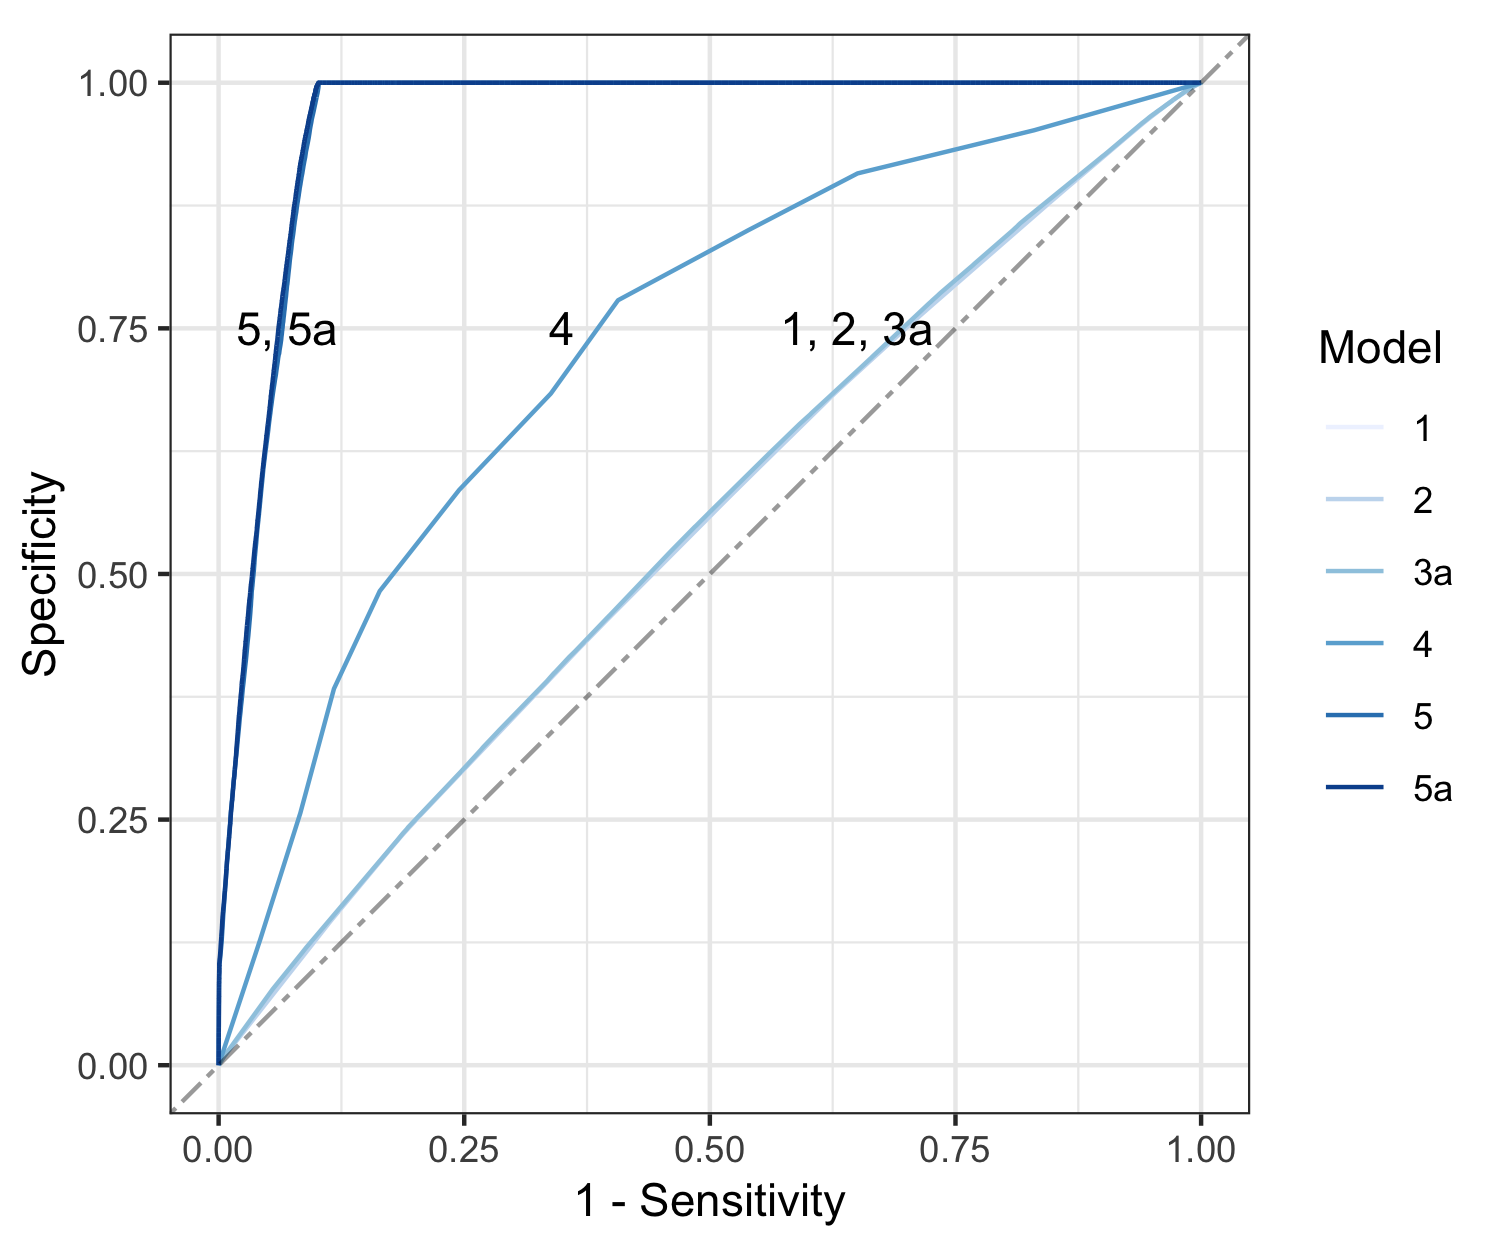
\includegraphics[width=0.6\linewidth]{/Users/tdounias/Desktop/Reed_Senior_Thesis/plots/roc_curves_indiv} 

}

\caption{ROC Curve for all individual models}\label{fig:roc the curves}
\end{figure}

In terms of trusting these results, I am confident in the results of
models 1, 3a, and 4, somewhat confident in model 5, and less so for
models 2, 3, and 5a. Models 2, 3 and 5a ``failed to converge''; this
means that the numeric approximation process by which \textit{R}
implements maximum likelihood estimation\footnote{Estimation of maximum
  likelihood here uses Adaptive Gaussian-Hermitian Quadrature (AGQ) to
  estimate coefficients {[}@handayani\_comparative\_2017{]}} for
coefficients doesn't give stable results, within certain conditions.
While model 5 did converge, it suffers from lack of variance in the
predictor for VBM, as explained in the beginning of this chapter; this
is the reason why the coefficient for mail vote is so disproportionately
large and variable. Model 6 simply did not run, even on a sub-sampled
dataset.

While I can't really derive any conclusions from this fact, there is a
distinct possibility that this either occurred due to a lack of
processing power, or lack of sufficient data for the model estimation to
even reach close to convergence. It is also important to point out that
model non-convergence is not a fatal issue in and of itself, but becomes
so if outputted coefficients wildly differ between calls of the model.
Running code to output 5-fold CV AUC involves estimating each model 5
times on different ``folds'', or sub-samples, of the dataset. During
this process the coefficients and AUC values remained fairly stable
between runs of the model, despite non-convergence. This leads me to
assume that the problem is significant, but not fatal for my models.

In terms of model fit, the models neatly fall into three groups based on
their cross-validated AUC. The first group, consisting of models 1, 2,
and 3a has an AUC of around \(.544\), making them only slightly
distinguishable from a coin-toss. This is fairly reasonable, since I am
building a model to make predictions at the ballot level while only
using county data or gender\footnote{Few counties wildly differ in their
  turnout percentages, and that the coefficient for male gender results
  in only around a 2.5\% decrease in voting probability}. The second
group based on AUC includes model 4, the only non-multilevel individual
model, with an AUC of around \(.733\), significantly outperforming the
first three models. Again, this is reasonable considering how wildly
different turnout is between election types; it is only natural that
these election-level variables would be so informative. The third group,
with the highest AUC of around \(.96\) are models 5 and 5a. This is a
direct result of the lack of variability in my data: Mail Voting is an
almost perfect predictor of the probability of voting.

There are two conclusions that can be derived from these results. None
of these conclusions are, sadly, related to my hypotheses on VBM. The
first is that the lack of variance in the data and a lack of processing
power are direct causes of my inability to estimate these models. This
is apparent in how model 6 does not run, other models do not converge,
and the coefficient for VBM is very large, since it doesn't vary enough
even after stratified sampling to account for any variance between mail
vote and conventional ballots. The second conclusion here is that,
despite these issues, there are some confirmable results on turnout in
general that are common between individual and county models. For
example, across models 2, 3, 3a the urban population of a county is a
substantial, negative factor in probability of voting, while the white
population is a very small, positive effect\footnote{This did, however,
  fail to reach statistical significance in both county and individual
  level models. This means that the small, positive effect is not that
  distinguishable from no effect at all.}. Similar conclusions can be
drawn for male gender, which is a very small negative effect in voting
probability as compared to female gender. These effects being stable
across several models mean that they are independent of the additions to
those models; for example, gender, urban population, and white
population have effects that are not accounted for when adding
individual level mixed effects. Despite not being able to assess VBM as
a factor of turnout probability, these models at least show that the
data does have substantial use for modelling at the individual level.

\begin{longtable}[]{@{}lccccccc@{}}
\caption{Estimated individual level coefficients (**Significant at the
.01 level *at the .05 level)
\label{tab:model_indiv_coef}}\tabularnewline
\toprule
\begin{minipage}[b]{0.12\columnwidth}\raggedright\strut
Predictor\strut
\end{minipage} & \begin{minipage}[b]{0.09\columnwidth}\centering\strut
Model 1\strut
\end{minipage} & \begin{minipage}[b]{0.10\columnwidth}\centering\strut
Model 2\strut
\end{minipage} & \begin{minipage}[b]{0.10\columnwidth}\centering\strut
Model 3\strut
\end{minipage} & \begin{minipage}[b]{0.10\columnwidth}\centering\strut
Model 3a\strut
\end{minipage} & \begin{minipage}[b]{0.10\columnwidth}\centering\strut
Model 4\strut
\end{minipage} & \begin{minipage}[b]{0.10\columnwidth}\centering\strut
Model 5\strut
\end{minipage} & \begin{minipage}[b]{0.10\columnwidth}\centering\strut
Model 5a\strut
\end{minipage}\tabularnewline
\midrule
\endfirsthead
\toprule
\begin{minipage}[b]{0.12\columnwidth}\raggedright\strut
Predictor\strut
\end{minipage} & \begin{minipage}[b]{0.09\columnwidth}\centering\strut
Model 1\strut
\end{minipage} & \begin{minipage}[b]{0.10\columnwidth}\centering\strut
Model 2\strut
\end{minipage} & \begin{minipage}[b]{0.10\columnwidth}\centering\strut
Model 3\strut
\end{minipage} & \begin{minipage}[b]{0.10\columnwidth}\centering\strut
Model 3a\strut
\end{minipage} & \begin{minipage}[b]{0.10\columnwidth}\centering\strut
Model 4\strut
\end{minipage} & \begin{minipage}[b]{0.10\columnwidth}\centering\strut
Model 5\strut
\end{minipage} & \begin{minipage}[b]{0.10\columnwidth}\centering\strut
Model 5a\strut
\end{minipage}\tabularnewline
\midrule
\endhead
\begin{minipage}[t]{0.12\columnwidth}\raggedright\strut
(Intercept)\strut
\end{minipage} & \begin{minipage}[t]{0.09\columnwidth}\centering\strut
-0.175\strut
\end{minipage} & \begin{minipage}[t]{0.10\columnwidth}\centering\strut
-0.042\strut
\end{minipage} & \begin{minipage}[t]{0.10\columnwidth}\centering\strut
0.001\strut
\end{minipage} & \begin{minipage}[t]{0.10\columnwidth}\centering\strut
0.001\strut
\end{minipage} & \begin{minipage}[t]{0.10\columnwidth}\centering\strut
-0.541**\strut
\end{minipage} & \begin{minipage}[t]{0.10\columnwidth}\centering\strut
-2.478**\strut
\end{minipage} & \begin{minipage}[t]{0.10\columnwidth}\centering\strut
-1.888**\strut
\end{minipage}\tabularnewline
\begin{minipage}[t]{0.12\columnwidth}\raggedright\strut
\strut
\end{minipage} & \begin{minipage}[t]{0.09\columnwidth}\centering\strut
(0.030)\strut
\end{minipage} & \begin{minipage}[t]{0.10\columnwidth}\centering\strut
(0.083)\strut
\end{minipage} & \begin{minipage}[t]{0.10\columnwidth}\centering\strut
(0.060)\strut
\end{minipage} & \begin{minipage}[t]{0.10\columnwidth}\centering\strut
(0.076)\strut
\end{minipage} & \begin{minipage}[t]{0.10\columnwidth}\centering\strut
(0.009)\strut
\end{minipage} & \begin{minipage}[t]{0.10\columnwidth}\centering\strut
(0.015)\strut
\end{minipage} & \begin{minipage}[t]{0.10\columnwidth}\centering\strut
(0.238)\strut
\end{minipage}\tabularnewline
\begin{minipage}[t]{0.12\columnwidth}\raggedright\strut
Pct\_urban\strut
\end{minipage} & \begin{minipage}[t]{0.09\columnwidth}\centering\strut
\strut
\end{minipage} & \begin{minipage}[t]{0.10\columnwidth}\centering\strut
-0.423**\strut
\end{minipage} & \begin{minipage}[t]{0.10\columnwidth}\centering\strut
-0.436**\strut
\end{minipage} & \begin{minipage}[t]{0.10\columnwidth}\centering\strut
-0.424**\strut
\end{minipage} & \begin{minipage}[t]{0.10\columnwidth}\centering\strut
\strut
\end{minipage} & \begin{minipage}[t]{0.10\columnwidth}\centering\strut
\strut
\end{minipage} & \begin{minipage}[t]{0.10\columnwidth}\centering\strut
-0.538**\strut
\end{minipage}\tabularnewline
\begin{minipage}[t]{0.12\columnwidth}\raggedright\strut
\strut
\end{minipage} & \begin{minipage}[t]{0.09\columnwidth}\centering\strut
\strut
\end{minipage} & \begin{minipage}[t]{0.10\columnwidth}\centering\strut
(0.055)\strut
\end{minipage} & \begin{minipage}[t]{0.10\columnwidth}\centering\strut
(0.059)\strut
\end{minipage} & \begin{minipage}[t]{0.10\columnwidth}\centering\strut
(0.062)\strut
\end{minipage} & \begin{minipage}[t]{0.10\columnwidth}\centering\strut
\strut
\end{minipage} & \begin{minipage}[t]{0.10\columnwidth}\centering\strut
\strut
\end{minipage} & \begin{minipage}[t]{0.10\columnwidth}\centering\strut
(0.114)\strut
\end{minipage}\tabularnewline
\begin{minipage}[t]{0.12\columnwidth}\raggedright\strut
Pct\_white\strut
\end{minipage} & \begin{minipage}[t]{0.09\columnwidth}\centering\strut
\strut
\end{minipage} & \begin{minipage}[t]{0.10\columnwidth}\centering\strut
0.067\strut
\end{minipage} & \begin{minipage}[t]{0.10\columnwidth}\centering\strut
0.075\strut
\end{minipage} & \begin{minipage}[t]{0.10\columnwidth}\centering\strut
0.073\strut
\end{minipage} & \begin{minipage}[t]{0.10\columnwidth}\centering\strut
\strut
\end{minipage} & \begin{minipage}[t]{0.10\columnwidth}\centering\strut
\strut
\end{minipage} & \begin{minipage}[t]{0.10\columnwidth}\centering\strut
-0.151\strut
\end{minipage}\tabularnewline
\begin{minipage}[t]{0.12\columnwidth}\raggedright\strut
\strut
\end{minipage} & \begin{minipage}[t]{0.09\columnwidth}\centering\strut
\strut
\end{minipage} & \begin{minipage}[t]{0.10\columnwidth}\centering\strut
(0.102)\strut
\end{minipage} & \begin{minipage}[t]{0.10\columnwidth}\centering\strut
(0.073)\strut
\end{minipage} & \begin{minipage}[t]{0.10\columnwidth}\centering\strut
(0.094)\strut
\end{minipage} & \begin{minipage}[t]{0.10\columnwidth}\centering\strut
\strut
\end{minipage} & \begin{minipage}[t]{0.10\columnwidth}\centering\strut
\strut
\end{minipage} & \begin{minipage}[t]{0.10\columnwidth}\centering\strut
(0.281)\strut
\end{minipage}\tabularnewline
\begin{minipage}[t]{0.12\columnwidth}\raggedright\strut
genderMale\strut
\end{minipage} & \begin{minipage}[t]{0.09\columnwidth}\centering\strut
\strut
\end{minipage} & \begin{minipage}[t]{0.10\columnwidth}\centering\strut
\strut
\end{minipage} & \begin{minipage}[t]{0.10\columnwidth}\centering\strut
-0.097**\strut
\end{minipage} & \begin{minipage}[t]{0.10\columnwidth}\centering\strut
-0.094**\strut
\end{minipage} & \begin{minipage}[t]{0.10\columnwidth}\centering\strut
\strut
\end{minipage} & \begin{minipage}[t]{0.10\columnwidth}\centering\strut
\strut
\end{minipage} & \begin{minipage}[t]{0.10\columnwidth}\centering\strut
0.094**\strut
\end{minipage}\tabularnewline
\begin{minipage}[t]{0.12\columnwidth}\raggedright\strut
\strut
\end{minipage} & \begin{minipage}[t]{0.09\columnwidth}\centering\strut
\strut
\end{minipage} & \begin{minipage}[t]{0.10\columnwidth}\centering\strut
\strut
\end{minipage} & \begin{minipage}[t]{0.10\columnwidth}\centering\strut
(0.007)\strut
\end{minipage} & \begin{minipage}[t]{0.10\columnwidth}\centering\strut
(0.007)\strut
\end{minipage} & \begin{minipage}[t]{0.10\columnwidth}\centering\strut
\strut
\end{minipage} & \begin{minipage}[t]{0.10\columnwidth}\centering\strut
\strut
\end{minipage} & \begin{minipage}[t]{0.10\columnwidth}\centering\strut
(0.017)\strut
\end{minipage}\tabularnewline
\begin{minipage}[t]{0.12\columnwidth}\raggedright\strut
Republican\strut
\end{minipage} & \begin{minipage}[t]{0.09\columnwidth}\centering\strut
\strut
\end{minipage} & \begin{minipage}[t]{0.10\columnwidth}\centering\strut
\strut
\end{minipage} & \begin{minipage}[t]{0.10\columnwidth}\centering\strut
\strut
\end{minipage} & \begin{minipage}[t]{0.10\columnwidth}\centering\strut
\strut
\end{minipage} & \begin{minipage}[t]{0.10\columnwidth}\centering\strut
\strut
\end{minipage} & \begin{minipage}[t]{0.10\columnwidth}\centering\strut
0.233**\strut
\end{minipage} & \begin{minipage}[t]{0.10\columnwidth}\centering\strut
0.208**\strut
\end{minipage}\tabularnewline
\begin{minipage}[t]{0.12\columnwidth}\raggedright\strut
\strut
\end{minipage} & \begin{minipage}[t]{0.09\columnwidth}\centering\strut
\strut
\end{minipage} & \begin{minipage}[t]{0.10\columnwidth}\centering\strut
\strut
\end{minipage} & \begin{minipage}[t]{0.10\columnwidth}\centering\strut
\strut
\end{minipage} & \begin{minipage}[t]{0.10\columnwidth}\centering\strut
\strut
\end{minipage} & \begin{minipage}[t]{0.10\columnwidth}\centering\strut
\strut
\end{minipage} & \begin{minipage}[t]{0.10\columnwidth}\centering\strut
(0.021)\strut
\end{minipage} & \begin{minipage}[t]{0.10\columnwidth}\centering\strut
(0.073)\strut
\end{minipage}\tabularnewline
\begin{minipage}[t]{0.12\columnwidth}\raggedright\strut
Other\strut
\end{minipage} & \begin{minipage}[t]{0.09\columnwidth}\centering\strut
\strut
\end{minipage} & \begin{minipage}[t]{0.10\columnwidth}\centering\strut
\strut
\end{minipage} & \begin{minipage}[t]{0.10\columnwidth}\centering\strut
\strut
\end{minipage} & \begin{minipage}[t]{0.10\columnwidth}\centering\strut
\strut
\end{minipage} & \begin{minipage}[t]{0.10\columnwidth}\centering\strut
\strut
\end{minipage} & \begin{minipage}[t]{0.10\columnwidth}\centering\strut
-0.085\strut
\end{minipage} & \begin{minipage}[t]{0.10\columnwidth}\centering\strut
-0.124\strut
\end{minipage}\tabularnewline
\begin{minipage}[t]{0.12\columnwidth}\raggedright\strut
\strut
\end{minipage} & \begin{minipage}[t]{0.09\columnwidth}\centering\strut
\strut
\end{minipage} & \begin{minipage}[t]{0.10\columnwidth}\centering\strut
\strut
\end{minipage} & \begin{minipage}[t]{0.10\columnwidth}\centering\strut
\strut
\end{minipage} & \begin{minipage}[t]{0.10\columnwidth}\centering\strut
\strut
\end{minipage} & \begin{minipage}[t]{0.10\columnwidth}\centering\strut
\strut
\end{minipage} & \begin{minipage}[t]{0.10\columnwidth}\centering\strut
(0.073)\strut
\end{minipage} & \begin{minipage}[t]{0.10\columnwidth}\centering\strut
(0.073)\strut
\end{minipage}\tabularnewline
\begin{minipage}[t]{0.12\columnwidth}\raggedright\strut
UAF\strut
\end{minipage} & \begin{minipage}[t]{0.09\columnwidth}\centering\strut
\strut
\end{minipage} & \begin{minipage}[t]{0.10\columnwidth}\centering\strut
\strut
\end{minipage} & \begin{minipage}[t]{0.10\columnwidth}\centering\strut
\strut
\end{minipage} & \begin{minipage}[t]{0.10\columnwidth}\centering\strut
\strut
\end{minipage} & \begin{minipage}[t]{0.10\columnwidth}\centering\strut
\strut
\end{minipage} & \begin{minipage}[t]{0.10\columnwidth}\centering\strut
-0.308**\strut
\end{minipage} & \begin{minipage}[t]{0.10\columnwidth}\centering\strut
0.325**\strut
\end{minipage}\tabularnewline
\begin{minipage}[t]{0.12\columnwidth}\raggedright\strut
\strut
\end{minipage} & \begin{minipage}[t]{0.09\columnwidth}\centering\strut
\strut
\end{minipage} & \begin{minipage}[t]{0.10\columnwidth}\centering\strut
\strut
\end{minipage} & \begin{minipage}[t]{0.10\columnwidth}\centering\strut
\strut
\end{minipage} & \begin{minipage}[t]{0.10\columnwidth}\centering\strut
\strut
\end{minipage} & \begin{minipage}[t]{0.10\columnwidth}\centering\strut
\strut
\end{minipage} & \begin{minipage}[t]{0.10\columnwidth}\centering\strut
(0.021)\strut
\end{minipage} & \begin{minipage}[t]{0.10\columnwidth}\centering\strut
(0.021)\strut
\end{minipage}\tabularnewline
\begin{minipage}[t]{0.12\columnwidth}\raggedright\strut
VBM\strut
\end{minipage} & \begin{minipage}[t]{0.09\columnwidth}\centering\strut
\strut
\end{minipage} & \begin{minipage}[t]{0.10\columnwidth}\centering\strut
\strut
\end{minipage} & \begin{minipage}[t]{0.10\columnwidth}\centering\strut
\strut
\end{minipage} & \begin{minipage}[t]{0.10\columnwidth}\centering\strut
\strut
\end{minipage} & \begin{minipage}[t]{0.10\columnwidth}\centering\strut
\strut
\end{minipage} & \begin{minipage}[t]{0.10\columnwidth}\centering\strut
23.764**\strut
\end{minipage} & \begin{minipage}[t]{0.10\columnwidth}\centering\strut
26.502**\strut
\end{minipage}\tabularnewline
\begin{minipage}[t]{0.12\columnwidth}\raggedright\strut
\strut
\end{minipage} & \begin{minipage}[t]{0.09\columnwidth}\centering\strut
\strut
\end{minipage} & \begin{minipage}[t]{0.10\columnwidth}\centering\strut
\strut
\end{minipage} & \begin{minipage}[t]{0.10\columnwidth}\centering\strut
\strut
\end{minipage} & \begin{minipage}[t]{0.10\columnwidth}\centering\strut
\strut
\end{minipage} & \begin{minipage}[t]{0.10\columnwidth}\centering\strut
\strut
\end{minipage} & \begin{minipage}[t]{0.10\columnwidth}\centering\strut
(45.255)\strut
\end{minipage} & \begin{minipage}[t]{0.10\columnwidth}\centering\strut
(285.774)\strut
\end{minipage}\tabularnewline
\begin{minipage}[t]{0.12\columnwidth}\raggedright\strut
Age\strut
\end{minipage} & \begin{minipage}[t]{0.09\columnwidth}\centering\strut
\strut
\end{minipage} & \begin{minipage}[t]{0.10\columnwidth}\centering\strut
\strut
\end{minipage} & \begin{minipage}[t]{0.10\columnwidth}\centering\strut
\strut
\end{minipage} & \begin{minipage}[t]{0.10\columnwidth}\centering\strut
\strut
\end{minipage} & \begin{minipage}[t]{0.10\columnwidth}\centering\strut
\strut
\end{minipage} & \begin{minipage}[t]{0.10\columnwidth}\centering\strut
0.093**\strut
\end{minipage} & \begin{minipage}[t]{0.10\columnwidth}\centering\strut
0.086**\strut
\end{minipage}\tabularnewline
\begin{minipage}[t]{0.12\columnwidth}\raggedright\strut
\strut
\end{minipage} & \begin{minipage}[t]{0.09\columnwidth}\centering\strut
\strut
\end{minipage} & \begin{minipage}[t]{0.10\columnwidth}\centering\strut
\strut
\end{minipage} & \begin{minipage}[t]{0.10\columnwidth}\centering\strut
\strut
\end{minipage} & \begin{minipage}[t]{0.10\columnwidth}\centering\strut
\strut
\end{minipage} & \begin{minipage}[t]{0.10\columnwidth}\centering\strut
\strut
\end{minipage} & \begin{minipage}[t]{0.10\columnwidth}\centering\strut
(0.009)\strut
\end{minipage} & \begin{minipage}[t]{0.10\columnwidth}\centering\strut
(0.009)\strut
\end{minipage}\tabularnewline
\begin{minipage}[t]{0.12\columnwidth}\raggedright\strut
typeGeneral\strut
\end{minipage} & \begin{minipage}[t]{0.09\columnwidth}\centering\strut
\strut
\end{minipage} & \begin{minipage}[t]{0.10\columnwidth}\centering\strut
\strut
\end{minipage} & \begin{minipage}[t]{0.10\columnwidth}\centering\strut
\strut
\end{minipage} & \begin{minipage}[t]{0.10\columnwidth}\centering\strut
\strut
\end{minipage} & \begin{minipage}[t]{0.10\columnwidth}\centering\strut
1.537**\strut
\end{minipage} & \begin{minipage}[t]{0.10\columnwidth}\centering\strut
\strut
\end{minipage} & \begin{minipage}[t]{0.10\columnwidth}\centering\strut
\strut
\end{minipage}\tabularnewline
\begin{minipage}[t]{0.12\columnwidth}\raggedright\strut
\strut
\end{minipage} & \begin{minipage}[t]{0.09\columnwidth}\centering\strut
\strut
\end{minipage} & \begin{minipage}[t]{0.10\columnwidth}\centering\strut
\strut
\end{minipage} & \begin{minipage}[t]{0.10\columnwidth}\centering\strut
\strut
\end{minipage} & \begin{minipage}[t]{0.10\columnwidth}\centering\strut
\strut
\end{minipage} & \begin{minipage}[t]{0.10\columnwidth}\centering\strut
(0.011)\strut
\end{minipage} & \begin{minipage}[t]{0.10\columnwidth}\centering\strut
\strut
\end{minipage} & \begin{minipage}[t]{0.10\columnwidth}\centering\strut
\strut
\end{minipage}\tabularnewline
\begin{minipage}[t]{0.12\columnwidth}\raggedright\strut
typeMidterm\strut
\end{minipage} & \begin{minipage}[t]{0.09\columnwidth}\centering\strut
\strut
\end{minipage} & \begin{minipage}[t]{0.10\columnwidth}\centering\strut
\strut
\end{minipage} & \begin{minipage}[t]{0.10\columnwidth}\centering\strut
\strut
\end{minipage} & \begin{minipage}[t]{0.10\columnwidth}\centering\strut
\strut
\end{minipage} & \begin{minipage}[t]{0.10\columnwidth}\centering\strut
0.829**\strut
\end{minipage} & \begin{minipage}[t]{0.10\columnwidth}\centering\strut
\strut
\end{minipage} & \begin{minipage}[t]{0.10\columnwidth}\centering\strut
\strut
\end{minipage}\tabularnewline
\begin{minipage}[t]{0.12\columnwidth}\raggedright\strut
\strut
\end{minipage} & \begin{minipage}[t]{0.09\columnwidth}\centering\strut
\strut
\end{minipage} & \begin{minipage}[t]{0.10\columnwidth}\centering\strut
\strut
\end{minipage} & \begin{minipage}[t]{0.10\columnwidth}\centering\strut
\strut
\end{minipage} & \begin{minipage}[t]{0.10\columnwidth}\centering\strut
\strut
\end{minipage} & \begin{minipage}[t]{0.10\columnwidth}\centering\strut
(0.011)\strut
\end{minipage} & \begin{minipage}[t]{0.10\columnwidth}\centering\strut
\strut
\end{minipage} & \begin{minipage}[t]{0.10\columnwidth}\centering\strut
\strut
\end{minipage}\tabularnewline
\begin{minipage}[t]{0.12\columnwidth}\raggedright\strut
typePrimary\strut
\end{minipage} & \begin{minipage}[t]{0.09\columnwidth}\centering\strut
\strut
\end{minipage} & \begin{minipage}[t]{0.10\columnwidth}\centering\strut
\strut
\end{minipage} & \begin{minipage}[t]{0.10\columnwidth}\centering\strut
\strut
\end{minipage} & \begin{minipage}[t]{0.10\columnwidth}\centering\strut
\strut
\end{minipage} & \begin{minipage}[t]{0.10\columnwidth}\centering\strut
-0.880**\strut
\end{minipage} & \begin{minipage}[t]{0.10\columnwidth}\centering\strut
\strut
\end{minipage} & \begin{minipage}[t]{0.10\columnwidth}\centering\strut
\strut
\end{minipage}\tabularnewline
\begin{minipage}[t]{0.12\columnwidth}\raggedright\strut
\strut
\end{minipage} & \begin{minipage}[t]{0.09\columnwidth}\centering\strut
\strut
\end{minipage} & \begin{minipage}[t]{0.10\columnwidth}\centering\strut
\strut
\end{minipage} & \begin{minipage}[t]{0.10\columnwidth}\centering\strut
\strut
\end{minipage} & \begin{minipage}[t]{0.10\columnwidth}\centering\strut
\strut
\end{minipage} & \begin{minipage}[t]{0.10\columnwidth}\centering\strut
(0.010)\strut
\end{minipage} & \begin{minipage}[t]{0.10\columnwidth}\centering\strut
\strut
\end{minipage} & \begin{minipage}[t]{0.10\columnwidth}\centering\strut
\strut
\end{minipage}\tabularnewline
\begin{minipage}[t]{0.12\columnwidth}\raggedright\strut
CV AUC\strut
\end{minipage} & \begin{minipage}[t]{0.09\columnwidth}\centering\strut
0.543\strut
\end{minipage} & \begin{minipage}[t]{0.10\columnwidth}\centering\strut
0.543\strut
\end{minipage} & \begin{minipage}[t]{0.10\columnwidth}\centering\strut
\strut
\end{minipage} & \begin{minipage}[t]{0.10\columnwidth}\centering\strut
0.545\strut
\end{minipage} & \begin{minipage}[t]{0.10\columnwidth}\centering\strut
0.733\strut
\end{minipage} & \begin{minipage}[t]{0.10\columnwidth}\centering\strut
0.961\strut
\end{minipage} & \begin{minipage}[t]{0.10\columnwidth}\centering\strut
0.963\strut
\end{minipage}\tabularnewline
\begin{minipage}[t]{0.12\columnwidth}\raggedright\strut
Obs\strut
\end{minipage} & \begin{minipage}[t]{0.09\columnwidth}\centering\strut
370,586\strut
\end{minipage} & \begin{minipage}[t]{0.10\columnwidth}\centering\strut
370,586\strut
\end{minipage} & \begin{minipage}[t]{0.10\columnwidth}\centering\strut
370,586\strut
\end{minipage} & \begin{minipage}[t]{0.10\columnwidth}\centering\strut
370,586\strut
\end{minipage} & \begin{minipage}[t]{0.10\columnwidth}\centering\strut
370,586\strut
\end{minipage} & \begin{minipage}[t]{0.10\columnwidth}\centering\strut
370,586\strut
\end{minipage} & \begin{minipage}[t]{0.10\columnwidth}\centering\strut
370,586\strut
\end{minipage}\tabularnewline
\begin{minipage}[t]{0.12\columnwidth}\raggedright\strut
Groups\strut
\end{minipage} & \begin{minipage}[t]{0.09\columnwidth}\centering\strut
64\strut
\end{minipage} & \begin{minipage}[t]{0.10\columnwidth}\centering\strut
64\strut
\end{minipage} & \begin{minipage}[t]{0.10\columnwidth}\centering\strut
64\strut
\end{minipage} & \begin{minipage}[t]{0.10\columnwidth}\centering\strut
64\strut
\end{minipage} & \begin{minipage}[t]{0.10\columnwidth}\centering\strut
64\strut
\end{minipage} & \begin{minipage}[t]{0.10\columnwidth}\centering\strut
64\strut
\end{minipage} & \begin{minipage}[t]{0.10\columnwidth}\centering\strut
64\strut
\end{minipage}\tabularnewline
\bottomrule
\end{longtable}


\end{document}
